\documentclass[11pt]{article}
\usepackage[utf8]{inputenc}
\usepackage[margin=1in]{geometry}
\usepackage[titletoc,title]{appendix}
\usepackage{fancyhdr}
\usepackage[T1]{fontenc}
\usepackage{courier}
\usepackage[colorlinks = true,linkcolor = blue]{hyperref}
\usepackage{amsmath,amsfonts,amssymb,mathtools}
\usepackage{graphicx,float}
\usepackage{subcaption}
\usepackage{minted}
\newminted{python}{frame=lines,framesep=2mm,baselinestretch=1.1,linenos}
\usepackage{changepage}

\pagestyle{fancy} \fancyhf{}
\lhead{Assignment 1} \rhead{AI502}
\rfoot{\thepage}
\title{Programming Assignment 1}
\author{20213073 Donggyu Kim}
\date{May 20, 2021}

\begin{document}
\maketitle
\thispagestyle{fancy}

\setcounter{section}{-1}
\section{Hyperparameters}
\begin{pythoncode*}{}
learning_rate = 0.001
num_epochs = 50
l_lambda = 0.01 #1e-5
\end{pythoncode*}
    I used the above hyperparameter set in every executions for fair comparison. Since our task is just a binary classification, I think 50 epoch is enough for a model to converge. \texttt{l\_lambda} is the weight for L1/L2 regularization: 0.01 for L2 and $10^{-5}$ for L1. The reason that I used the different values is described in Section \ref{L1}.

\section{Classification Model}
\setcounter{subsection}{-1}
\subsection{Setting}
\begin{pythoncode*}{}
optimizer = torch.optim.SGD(model.parameters(), lr=learning_rate,\
                                                momentum=0.9)
\end{pythoncode*}
    To compare the three classification models under the same condition, I equally used the above SGD with Momentum optimizer, without regularization (though the given VGG and ResNet models use Batch Normalization, which has inherent regularization effect).

\subsection{MLP}\label{vanilla}
    \begin{figure}[H]
        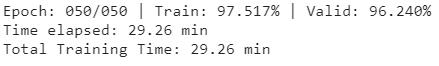
\includegraphics[width=0.8\linewidth]{img/MLP/final.PNG}
        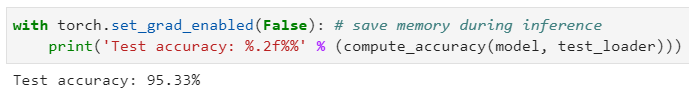
\includegraphics[width=1\linewidth]{img/MLP/test.PNG}
        \caption{Training result of MLP}
        \label{fig1}
    \end{figure}
    This is the result of training MLP for 50 epochs. It took 29.26 minutes and gets 97.52\%/96.24\%/95.33\% of train/valid/test accuracy. See Fig \ref{fig4} for its train loss and train/validation accuracy curves.\\
    Let's call this \textit{vanilla MLP} for further comparisons in the regularization and optimization sections.

\subsection{VGG-16}
    \begin{figure}[H]
        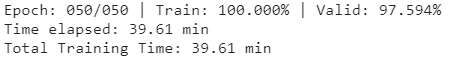
\includegraphics[width=0.8\linewidth]{img/VGG/final.PNG}
        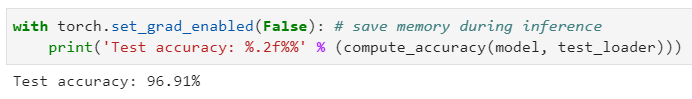
\includegraphics[width=1\linewidth]{img/VGG/test.PNG}
        \caption{Training result of VGG-16}
        \label{fig2}
    \end{figure}
    VGGNet has several variants according to the number of layers. I chose VGG-16 among them. As Fig \ref{fig2} shows, VGG-16 took 39.61 minutes for training, and after 50 epochs, it has 100.0\%/97.59\%/96.91\% of train/valid/test accuracy. VGG-16 took more time but get better accuracy compare to MLP. See Fig \ref{fig4} for its train loss and train/validation accuracy curves.

\subsection{ResNet-18}
    \begin{figure}[H]
        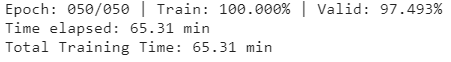
\includegraphics[width=0.8\linewidth]{img/Res/final.PNG}
        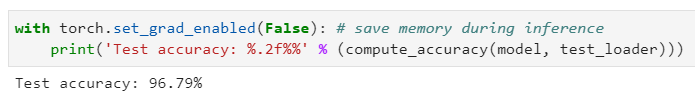
\includegraphics[width=1\linewidth]{img/Res/test.PNG}
        \caption{Training result of ResNet-18}
        \label{fig3}
    \end{figure}
    ResNet also has several variants, but the instruction specified ResNet-18. As Fig \ref{fig3} shows, ResNet-18 took 65.31 minutes for training. After 50 epochs, it has 100.0\%/97.49\%/96.79\% of train/valid/test accuracy. It took more time compare to VGG-16 but get a bit lower validation and test accuracies. See Fig \ref{fig4} for its train loss and train/valid accuracy curves.

\subsection{Comparison}\label{model}
    \begin{figure}[H]
        \begin{subfigure}[H]{1\textwidth}
            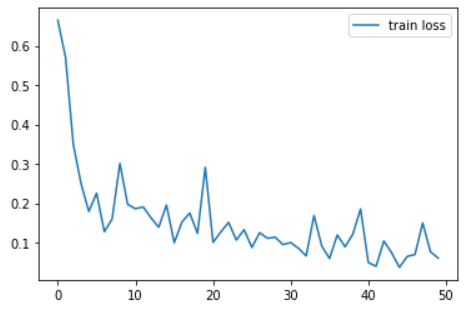
\includegraphics[width=0.5\linewidth]{img/MLP/loss.PNG}
            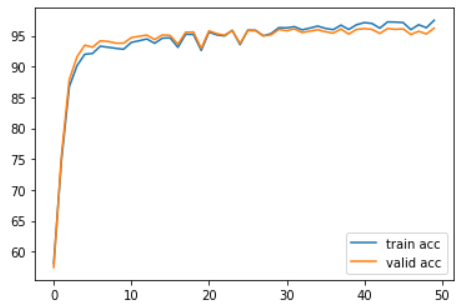
\includegraphics[width=0.5\linewidth]{img/MLP/acc.PNG}
            \caption{MLP}\vspace{2mm}
        \end{subfigure}
        \begin{subfigure}[H]{1\textwidth}
            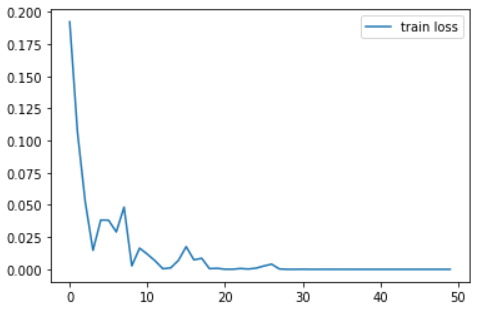
\includegraphics[width=0.5\linewidth]{img/VGG/loss.PNG}
            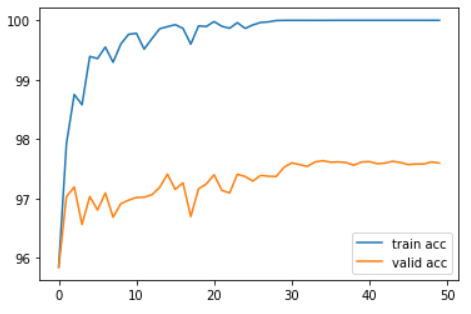
\includegraphics[width=0.5\linewidth]{img/VGG/acc.PNG}
            \caption{VGG-16}\vspace{2mm}
        \end{subfigure}
        \begin{subfigure}[H]{1\textwidth}
            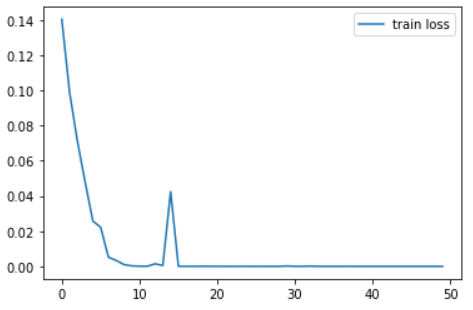
\includegraphics[width=0.5\linewidth]{img/Res/loss.PNG}
            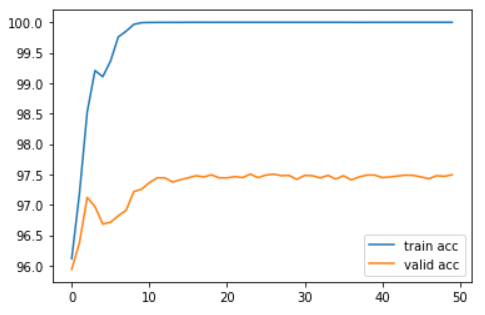
\includegraphics[width=0.5\linewidth]{img/Res/acc.PNG}
            \caption{ResNet-18}
        \end{subfigure}
        \caption{Loss and accuracy curves}
        \label{fig4}
    \end{figure}
    Both MLP and the CNN models show very high accuracy. Also, there is no sign of overfitting, at least for the 50 epochs. This should be because the task is too easy - binary classification.
    Though, MLP showed significant differences with the CNN models. It has higher training loss and lower train/validation accuracy in the first few epochs; MLP had about 50\% accuracy while VGG-16 and ResNet-18 reached 90\% in their first epoch. Also, MLP has almost same training and validation accuracies, while the CNN models show about 3\% gap between them. This can be the evidence that the CNN models learns better from the training data. On the other hand, VGG-16 and ResNet-18 does not differ so much. Although ResNet-18 has lower training loss in the first few epochs, the loss converges to almost 0 for both of them at the end. Interesting point is that ResNet-18 has smoother accuracy curves. I guess this is because the skip connection has stabilizing effect in the training.

\section{Regularization}
\setcounter{subsection}{-1}
\subsection{Setting}
    In this part, MLP is used as the base model and SGD with Momentum is used as the optimizer. The given VGG and ResNet are using Batch Normalization, which already has regularization effect. Furthermore, Dropout is used on FC layers in general, but the given CNN models are using Average Pooling instead of FC layers. This is why I chose MLP as the base model to compare the regularization methods.

\subsection{Dropout}
\begin{pythoncode*}{}
class MLP(nn.Module):
    def __init__(self, drop = 0):
        super().__init__()
        layers = []
        in_dim = 3*32*32
        for dim in [1024, 512, 256, 128]:
            out_dim = dim
            layers.append(nn.Linear(in_dim, out_dim))
            if drop > 0:
                layers.append(nn.Dropout(drop))
            layers.append(nn.ReLU())
            in_dim = out_dim
        layers.append(nn.Linear(out_dim, 2))
        self.network = nn.Sequential(*layers)
\end{pythoncode*}
    I added the parameter \texttt{drop}, a Dropout rate, to construct MLP with Dropout. If \texttt{drop} is bigger than 0, each layer of the MLP performs Dropout.
\begin{pythoncode*}{}
model = mlp.MLP(drop=0.5)
\end{pythoncode*}
    Dropout rate is set to 0.5 in general, so I also used 0.5 here.
    \begin{figure}[H]
        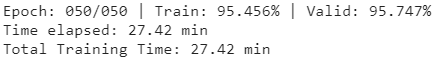
\includegraphics[width=0.8\linewidth]{img/Dropout/final.PNG}
        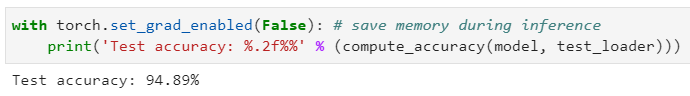
\includegraphics[width=1\linewidth]{img/Dropout/test.PNG}
        \caption{Training result of MLP with Dropout}
        \label{fig5}
    \end{figure}
    This is the result of training MLP with Dropout for 50 epochs. It took 27.42 minutes and gets 95.46\%/95.75\%/94.89\% of train/valid/test accuracy. Since regularization is to avoid overfitting of a model and get better results for unseen (test) data, it is quite disappointing that MLP with Dropout did not beat vanilla MLP's test accuracy. Though, it is comforting that MLP with Dropout has almost same training and validation accuracies. See Fig \ref{fig11} for its train loss and train/validation accuracy curves.
    
\subsection{L2 Regularization}
\begin{pythoncode*}{}
optimizer = torch.optim.SGD(model.parameters(), lr=learning_rate,\
                                momentum=0.9, weight_decay=l_lambda)
\end{pythoncode*}
    It is possible to implement L2 regularization explicitly, but is is simply done by assigning \texttt{weight\_decay} value. As I mentioned at the very first of this document, I set \texttt{l\_lambda} to 0.01 for L2 regularization.
    \begin{figure}[H]
        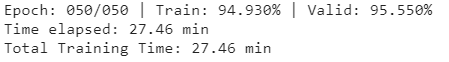
\includegraphics[width=0.8\linewidth]{img/L2/final.PNG}
        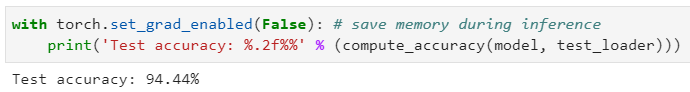
\includegraphics[width=1\linewidth]{img/L2/test.PNG}
        \caption{Training result of MLP with L2 regularization}
        \label{fig6}
    \end{figure}
    This is the result of training MLP with L2 regularization for 50 epochs. It took 27.46 minutes and gets 94.93\%/95.55\%/94.44\% of train/valid/test accuracy. It is quite surprising that the validation accuracy is higher than the training accuracy. Same as Dropout, MLP with L2 regularization did not beat vanilla MLP. See Fig \ref{fig11} for its train loss and train/validation accuracy curves. To check whether L2 regularization worked well or not, I plotted L2 norm changes for each model (Fig \ref{fig9}).

\subsection{L1 Regularization}\label{L1}
\begin{pythoncode*}{}
l1_norm = sum(torch.norm(param, p=1) for param in model.parameters())
l2_norm = sum(torch.norm(param) for param in model.parameters())
cost += l_lambda * l1_norm
\end{pythoncode*}
    There is no implicit L1 regularization option in the optimizer. Therefore, I added the above code for L1 regularization. The first 2 lines compute L1 and L2 norms of each model, and the results are in Fig. \ref{fig9} and Fig. \ref{fig10}. The last line must be commented out when the model is not using L1 regularization.
    \begin{figure}[H]\centering
        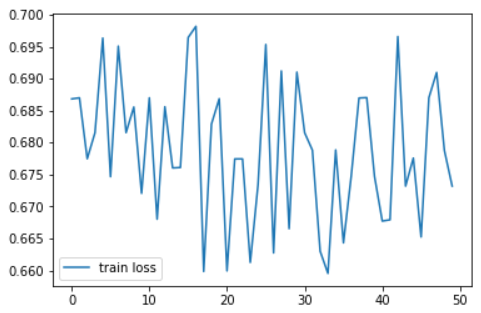
\includegraphics[width=0.7\linewidth]{img/L1/fail_loss.PNG}
        \caption{MLP with L1 regularization failed to converge}
        \label{fig7}
    \end{figure}
    As in L2 regularization, I first used \texttt{l\_lambda} value 0.01 for L1 regularization. However, the model did not converged well (Fig. \ref{fig7}) and got only 57\% of training accuracy. This is because L1 norm is too large ($>10^{5}$) compare to the prediction loss term, so the model only decreased its weights not the training loss. Thus, I changed \texttt{l\_lambda} value to $10^{-5}$ and got the appropriate result this time.
    \begin{figure}[H]
        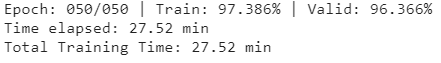
\includegraphics[width=0.8\linewidth]{img/L1/final.PNG}
        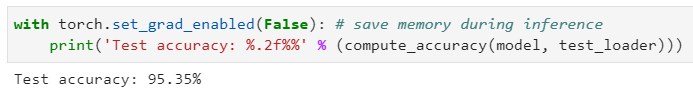
\includegraphics[width=1\linewidth]{img/L1/test.PNG}
        \caption{Training result of MLP with L1 regularization}
        \label{fig8}
    \end{figure}
    This is the result of training MLP with L1 regularization for 50 epochs. It took 27.52 minutes and gets 97.39\%/96.37\%/95.35\% of train/valid/test accuracy. Dropout and L2 regularization did not beat vanilla MLP, but L1 regularization slightly beat vanilla MLP's test accuracy. See Fig \ref{fig11} for its train loss and train/validation accuracy curves. To check whether L1 regularization worked well or not, I plotted L1 norm changes for each model (Fig \ref{fig10}).

\subsection{Comparison}\label{regularization}
    \begin{figure}[H]
        \begin{subfigure}[H]{0.5\textwidth}
            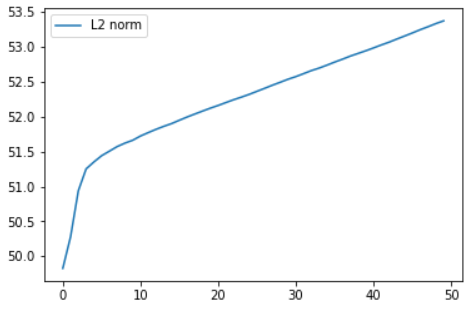
\includegraphics[width=1\linewidth]{img/MLP/l2.PNG}
            \caption{Vanilla (No regularization)}\vspace{2mm}
        \end{subfigure}
        \begin{subfigure}[H]{0.5\textwidth}
            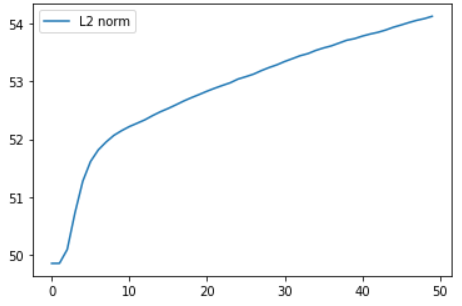
\includegraphics[width=1\linewidth]{img/Dropout/l2.PNG}
            \caption{Dropout}\vspace{2mm}
        \end{subfigure}
        \begin{subfigure}[H]{0.5\textwidth}
            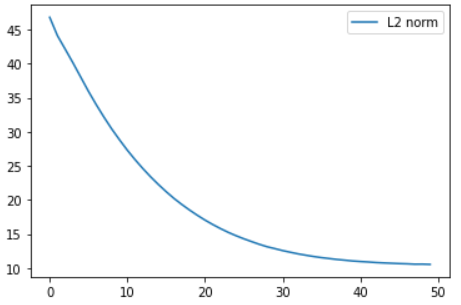
\includegraphics[width=1\linewidth]{img/L2/l2.PNG}\caption{L2}
        \end{subfigure}
        \begin{subfigure}[H]{0.5\textwidth}
            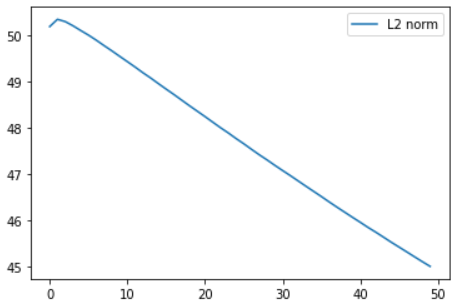
\includegraphics[width=1\linewidth]{img/L1/l2.PNG}\caption{L1}
        \end{subfigure}
        \caption{L2 norm}
        \label{fig9}
    \end{figure}
    While L2 norm increases for vanilla MLP and MLP with Dropout as training goes on, L2 regularization significantly reduced L2 norm. L1 regularization also leads to decrease in L2 norm.
    \begin{figure}[H]
        \begin{subfigure}[H]{0.5\textwidth}
            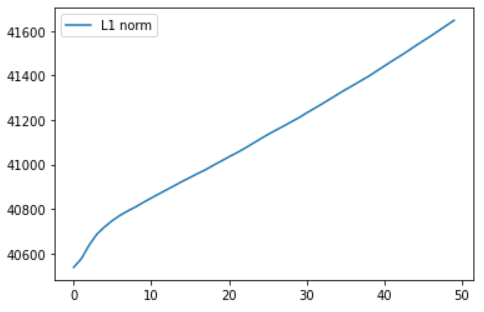
\includegraphics[width=1\linewidth]{img/MLP/l1.PNG}
            \caption{Vanilla (No regularization)}\vspace{2mm}
        \end{subfigure}
        \begin{subfigure}[H]{0.5\textwidth}
            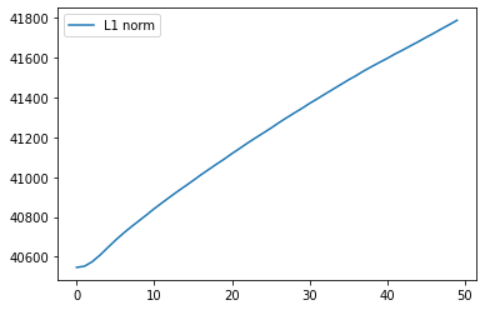
\includegraphics[width=1\linewidth]{img/Dropout/l1.PNG}
            \caption{Dropout}\vspace{2mm}
        \end{subfigure}
        \begin{subfigure}[H]{0.5\textwidth}
            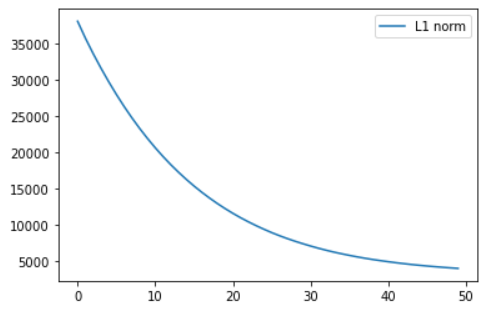
\includegraphics[width=1\linewidth]{img/L2/l1.PNG}\caption{L2}
        \end{subfigure}
        \begin{subfigure}[H]{0.5\textwidth}
            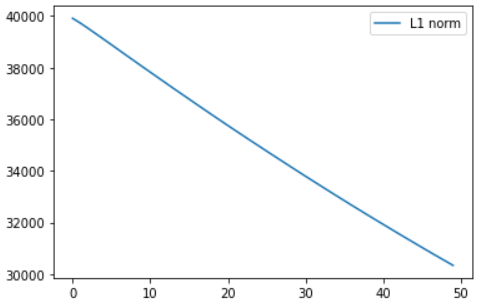
\includegraphics[width=1\linewidth]{img/L1/l1.PNG}\caption{L1}
        \end{subfigure}
        \caption{L1 norm}
        \label{fig10}
    \end{figure}
    While L1 norm increases for vanilla MLP and MLP with Dropout as training goes on, L1 regularization significantly reduced L1 norm. L2 regularization also leads to decrease in L1 norm. As I previously mentioned, L1 norm is very large so deciding \texttt{l\_lambda} should take this into account.
    \begin{figure}[H]
        \begin{subfigure}[H]{1\textwidth}
            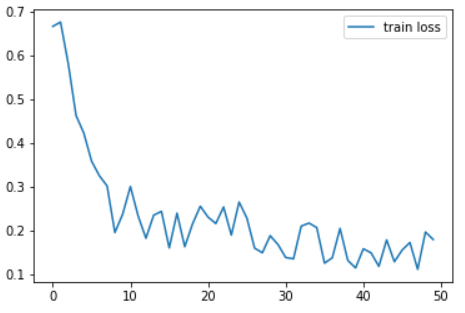
\includegraphics[width=0.5\linewidth]{img/Dropout/loss.PNG}
            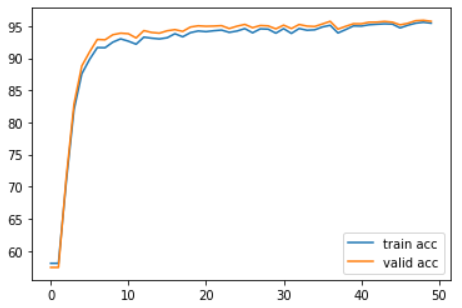
\includegraphics[width=0.5\linewidth]{img/Dropout/acc.PNG}
            \caption{Dropout}\vspace{2mm}
        \end{subfigure}
        \begin{subfigure}[H]{1\textwidth}
            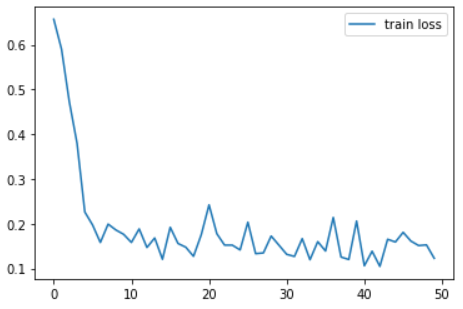
\includegraphics[width=0.5\linewidth]{img/L2/loss.PNG}
            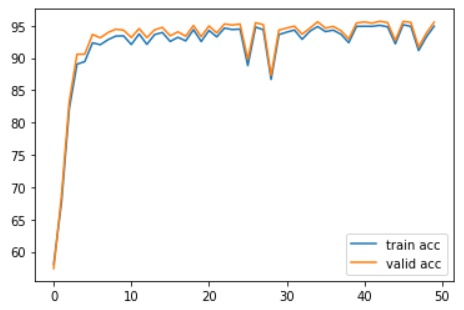
\includegraphics[width=0.5\linewidth]{img/L2/acc.PNG}
            \caption{L2}\vspace{2mm}
        \end{subfigure}
        \begin{subfigure}[H]{1\textwidth}
            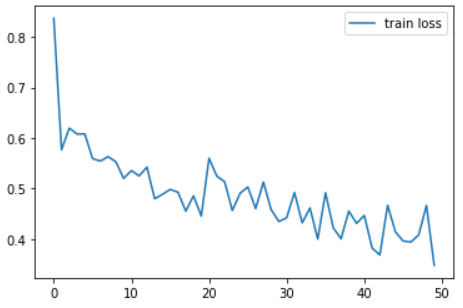
\includegraphics[width=0.5\linewidth]{img/L1/loss.PNG}
            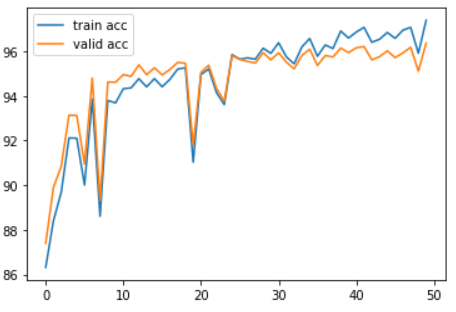
\includegraphics[width=0.5\linewidth]{img/L1/acc.PNG}
            \caption{L1}
        \end{subfigure}
        \caption{Loss and accuracy curves}
        \label{fig11}
    \end{figure}
    Compare to the result in Fig. \ref{fig4} (a), Dropout does not show any significant differences while L1 and L2 regularization shows a bit noisy accuracy curves. I think this is because weight decaying disturbs the model for regularization, while Dropout stabilizes the model by the bagging effect.

\section{Optimization}
\setcounter{subsection}{-1}
\subsection{Setting}
    In this part, MLP is used as the base model, without regularization.
    
\subsection{Momentum}
    This is vanilla MLP that I've already discussed. See Section \ref{vanilla} for the result.

\subsection{AdaGrad}
\begin{pythoncode*}{}
optimizer = torch.optim.Adagrad(model.parameters(), lr=learning_rate)
\end{pythoncode*}
    This time, the MLP is trained with AdaGrad optimizer.
    \begin{figure}[H]
        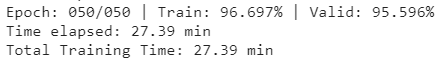
\includegraphics[width=0.8\linewidth]{img/AdaGrad/final.PNG}
        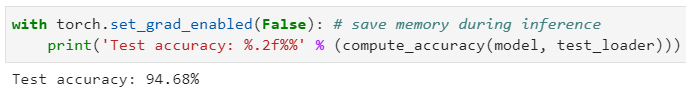
\includegraphics[width=1\linewidth]{img/AdaGrad/test.PNG}
        \caption{Training result of MLP with AdaGrad optimizer}
        \label{fig12}
    \end{figure}
    This is the result of training MLP for 50 epochs. It took 27.39 minutes and gets 96.70\%/95.60\%/94.68\% of train/valid/test accuracy. See Fig \ref{fig14} for its train loss and train/validation accuracy curves.
    
\subsection{Adam}
\begin{pythoncode*}{}
optimizer = torch.optim.Adam(model.parameters(), lr=learning_rate)
\end{pythoncode*}
    This time, the MLP is trained with AdaGrad optimizer.
    \begin{figure}[H]
        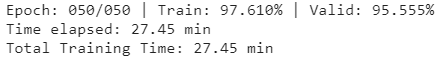
\includegraphics[width=0.8\linewidth]{img/Adam/final.PNG}
        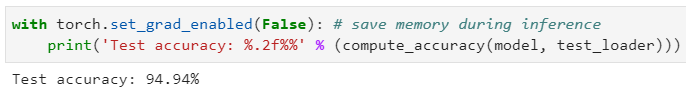
\includegraphics[width=1\linewidth]{img/Adam/test.PNG}
        \caption{Training result of MLP with Adam optimizer}
        \label{fig13}
    \end{figure}
    This is the result of training MLP for 50 epochs. It took 27.45 minutes and gets 97.61\%/95.56\%/94.94\% of train/valid/test accuracy. See Fig \ref{fig14} for its train loss and train/validation accuracy curves.

\subsection{Comparison}\label{optimization}
    \begin{figure}[H]
        \begin{subfigure}[H]{1\textwidth}
            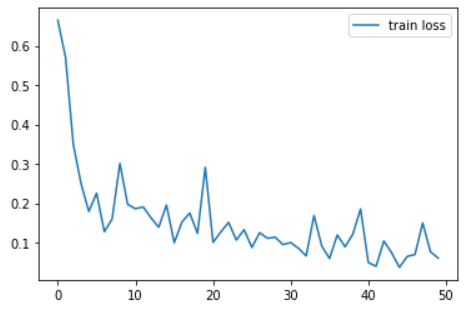
\includegraphics[width=0.5\linewidth]{img/MLP/loss.PNG}
            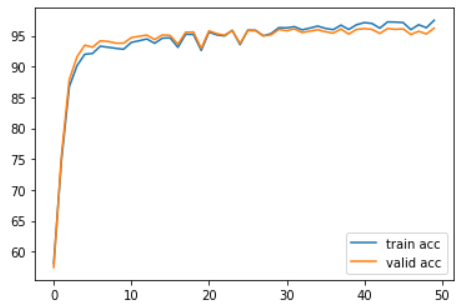
\includegraphics[width=0.5\linewidth]{img/MLP/acc.PNG}
            \caption{Momentum}\vspace{2mm}
        \end{subfigure}
        \begin{subfigure}[H]{1\textwidth}
            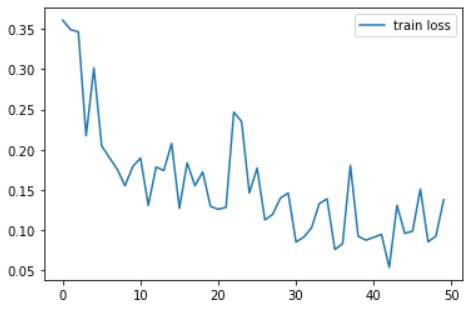
\includegraphics[width=0.5\linewidth]{img/AdaGrad/loss.PNG}
            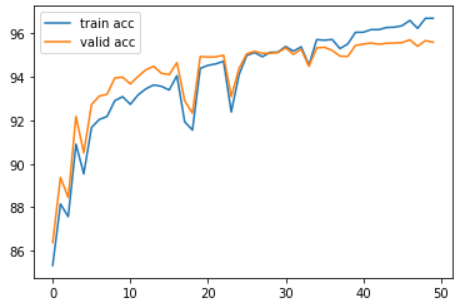
\includegraphics[width=0.5\linewidth]{img/AdaGrad/acc.PNG}
            \caption{AdaGrad}\vspace{2mm}
        \end{subfigure}
        \begin{subfigure}[H]{1\textwidth}
            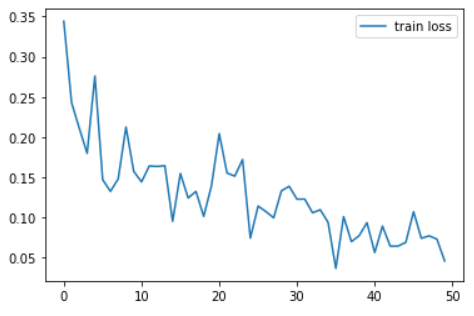
\includegraphics[width=0.5\linewidth]{img/Adam/loss.PNG}
            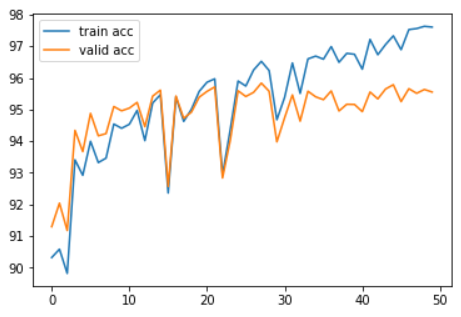
\includegraphics[width=0.5\linewidth]{img/Adam/acc.PNG}
            \caption{Adam}
        \end{subfigure}
        \caption{Loss and accuracy curves}
        \label{fig14}
    \end{figure}
    AdaGrad adapts the learning rates of the model parameters by scaling them inversely proportional to the square root of the sum of all their historical. Therefore, the model is trained very fast in the first few epochs and got up to 90\% accuracy. However, shrinking the learning rate based on the entire history of the gradient makes the learning rate too small. It appears directly after 5 epochs. Adam is a combination of RMSProp and momentum. The learning rate is bounded, and so the model's training accuracy increased continuously.
    
\end{document}
